%- HandOut Flag -----------------------------------------------------------------------------------------
\newif\ifHandout

%- D0cum3nt ----------------------------------------------------------------------------------------------
\documentclass[beamer,10pt]{standalone}   
%\documentclass[beamer,10pt,handout]{standalone}  \Handouttrue  

%- HandOut Flag -----------------------------------------------------------------------------------------
\ifHandout
	\setbeameroption{show notes} %print notes   
\fi

	
%- Packages ----------------------------------------------------------------------------------------------
\usepackage{custom-style}
\usetikzlibrary{positioning}
\usepackage{multicol}


%--Beamer Style-----------------------------------------------------------------------------------------------
\usetheme{toninus}
\usepackage{animate}
\usetikzlibrary{positioning, arrows}
\usetikzlibrary{shapes}

\begin{document}
%-------------------------------------------------------------------------------------------------------------------------------------------------
\begin{frame}{Introduction}
	\begin{columns}[]
	\begin{column}{0.55\textwidth}
		PhD colloquium:
		\\
		i.e.~
		\emph{a talk inspired by my doctoral project}

	\vspace{1em}

	\begin{itemize}
		\item<2-> \underline{Thesis}: focus on certain \emph{higher generalizations} in \emph{ symplectic geometry}.
		\item<3-> \underline{Talk}: focus on \emph{motivations} rather than details.
	\end{itemize}	



	\end{column}
	\begin{column}{0.4\textwidth}
		\onslide<2->{
			\fbox{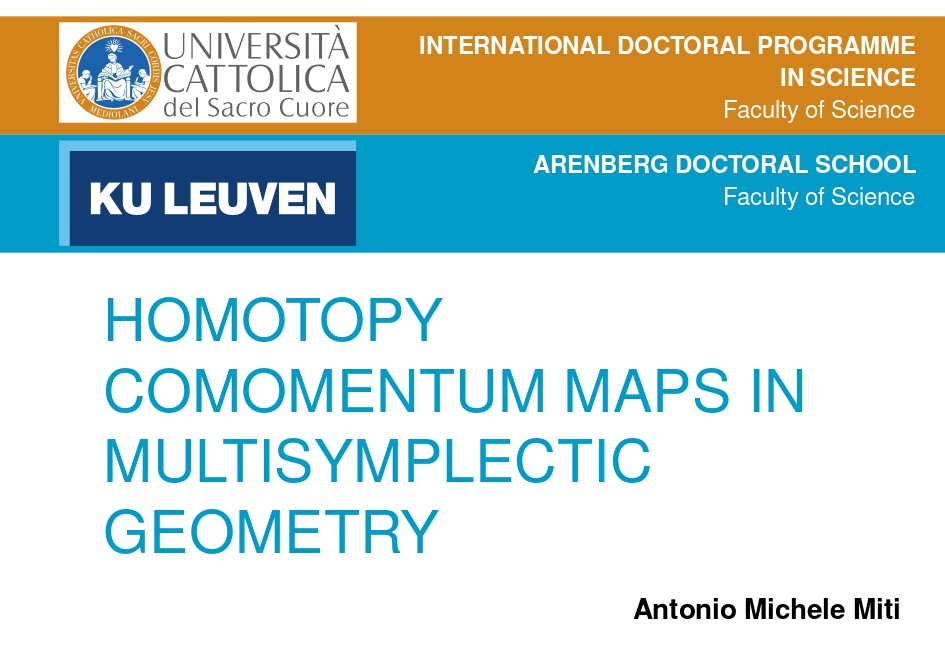
\includegraphics[width=.9\textwidth]{Pictures/thesis-zoom}}
		}
	\end{column}
	\end{columns}

	\vfill

	\vfill
	\begin{columns}[]
	\begin{column}{0.35\textwidth}
		\onslide<4->{
			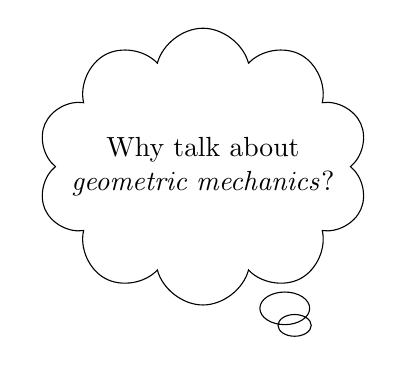
\begin{tikzpicture}
				\node [draw,cloud callout, minimum height=10em,minimum width=12em] (L1) {};
				\node [text width=12em,text centered] (L2) {Why talk about \\ \emph{geometric mechanics}?};
			\end{tikzpicture}
		}
	\end{column}
	\begin{column}{0.65\textwidth}
		\onslide<5->{
			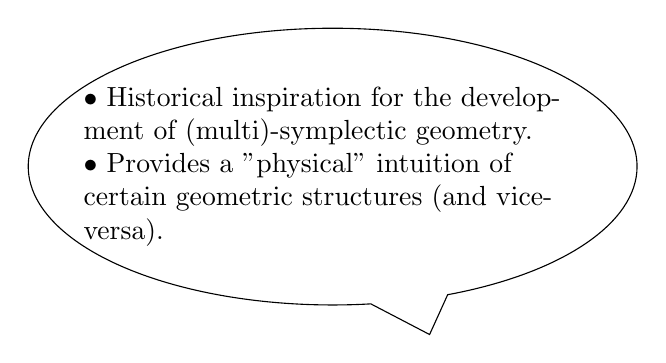
\begin{tikzpicture}
				\node [draw,ellipse callout, minimum height=10em,minimum width=22em] (L1) {};
				\node [text width=18em] (L2) 
					{
						$\bullet$ Historical inspiration for the development of (multi)-symplectic geometry.
						\\
						$\bullet$ Provides a "physical" intuition of certain geometric structures (and vice-versa).
					};
			\end{tikzpicture}
		}
	\end{column}
	\end{columns}



\end{frame}
\note[itemize]{
	\item
}
%-------------------------------------------------------------------------------------------------------------------------------------------------

\outline

\subsection{Geometry \& Physics}
%-------------------------------------------------------------------------------------------------------------------------------------------------
\begin{frame}[t,fragile]{What is... mechanics?}
	\begin{center}
		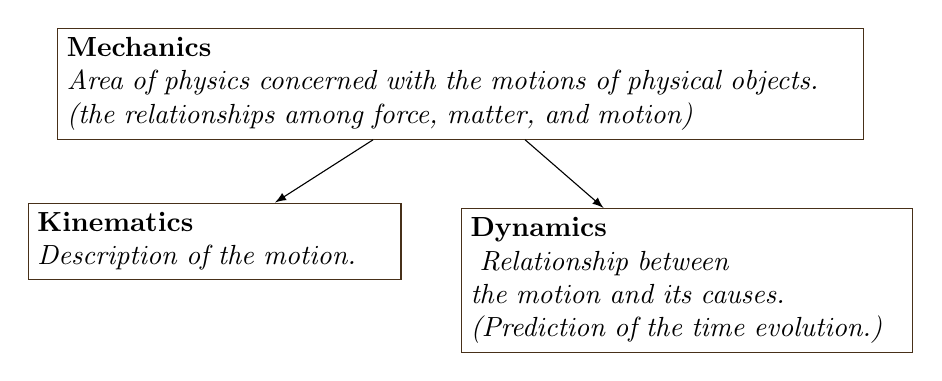
\begin{tikzpicture}
		 	\node[draw=orange!20!black!90,right,text width=10cm] (s1) at (0,0)
		    {
				{\bf Mechanics} \\
				\emph{Area of physics concerned with the motions of physical objects.\\
				(the relationships among force, matter, and motion)}		            
		     }; 
 			\node[draw=orange!20!black!90,text width=4.5cm] (t1) at (2cm,-2cm)
    		{
		   		{\bf Kinematics}
		   		\\ \emph{Description of the motion.}
	        };	
 			\node[draw=orange!20!black!90,text width=5.5cm] (t2) at (8cm,-2.5cm)
    			{
		    		{\bf Dynamics} \\
		   			\emph{ Relationship between\\ the motion and its causes.\\ (Prediction of the time evolution.)}
	        };
	        \draw[-latex] (s1) -- (t1);
        	\draw[-latex] (s1) -- (t2);
		\end{tikzpicture}
	\end{center}

	\vfill
	\begin{columns}
    	\begin{column}{.33\textwidth}
	   		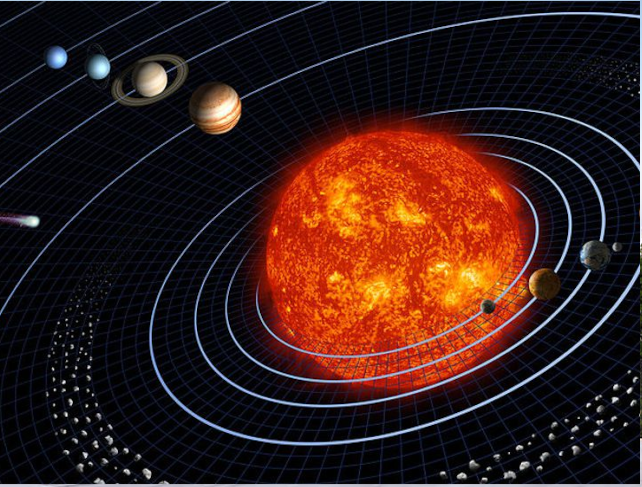
\includegraphics[width=\textwidth]{Pictures/solar} 	
		\end{column}
    	\begin{column}{.33\textwidth}
	   		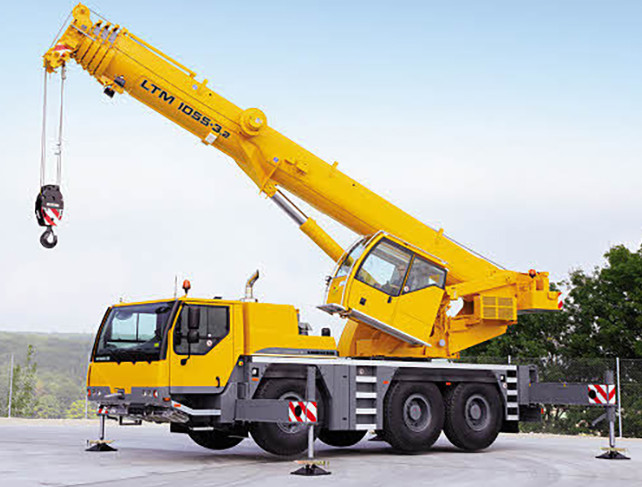
\includegraphics[width=\textwidth]{Pictures/autogru-liebherr} 	
		\end{column}
    	\begin{column}{.33\textwidth}
	   		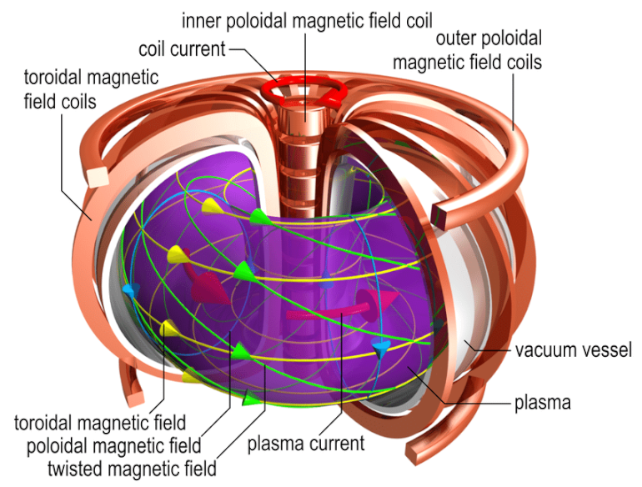
\includegraphics[width=\textwidth]{Pictures/plasma} 	
		\end{column}
	\end{columns}
\end{frame}
\note[itemize]{
	\item
}
%-------------------------------------------------------------------------------------------------------------------------------------------------

%-------------------------------------------------------------------------------------------------------------------------------------------------
\begin{frame}[t]{How does Geometry gets into Physics?}
	%
	\begin{block}{Trivial answer:}
		It appears in describing the "physical space" in which all "physical systems" are embedded.
	\end{block}
	\vfill

  	\begin{columns}<2->
  		\hfill
    	\begin{column}{.6\textwidth}
    		\begin{block}{Historical fact:}
				Measuring "Earth" is one of the oldest problem in mathematics.
			\end{block}
    	\end{column}
    	\begin{column}{.3\textwidth}
			\center
			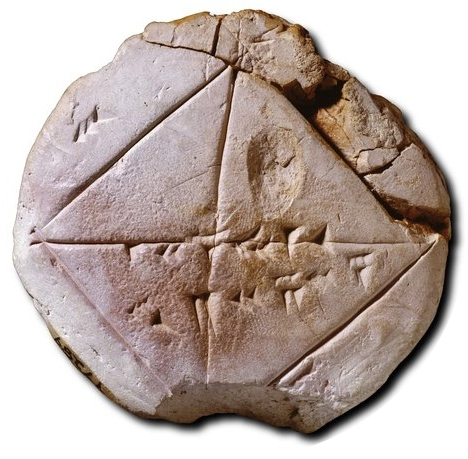
\includegraphics[width=0.5\textwidth]{Pictures/babylon-tablet} 		
    	\end{column}
    \end{columns}
    %
    \vspace*{-.5em}    
  	\begin{columns}<3->
  		\hfill
    	\begin{column}{.3\textwidth}
    		\center
			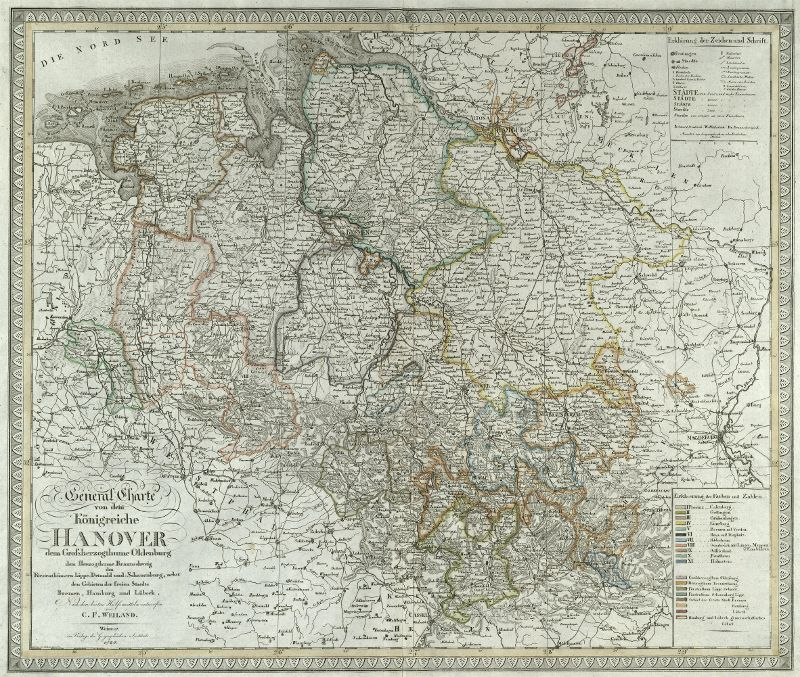
\includegraphics[width=0.8\textwidth]{Pictures/hannover-map} 		
    	\end{column}
    	\begin{column}{.6\textwidth}
				Also modern (intrinsic) differential geometry stemmed from cartography!
				\\
				\small (a cartographic survey of the Kingdom of Hanover commissioned to Carl Friederich Gauss in 1828.)	    			
		\end{column}
    \end{columns}    
    
    
	\vfill
	\begin{alertblock}<4->{There is much more!}
		Geometry provides a powerful language to encode deep properties of physics encompassing a huge variety of mechanical systems.
	\end{alertblock}
\end{frame}
\note[itemize]{
	\item Three fundamentals concepts: Space, Body (system), Displacement.
	\item Nevertheless, the problem of measuring "Earth" is one of the oldest problem in mathematics (see \url{https://en.wikipedia.org/wiki/YBC_7289})
	\item YBC 7289 is a Babylonian clay tablet notable for containing an accurate sexagesimal approximation to the square root of 2, the length of the diagonal of a unit square. 
	\item Nel 1818 fu chiesto a Gauss di compiere la rilevazione geodetica del Regno di Hannover, associandola ai precedenti rilevamenti effettuati in Danimarca.
La cartografia dell'Hannover portò Gauss a sviluppare la geometria differenziale insieme alle potenzialità della geometria non euclidea.
}
%-------------------------------------------------------------------------------------------------------------------------------------------------

%-------------------------------------------------------------------------------------------------------------------------------------------------
\subsection{Geometric mechanics in a nutshell}
\begin{frame}{What we mean by: \emph{Geometric mechanics}? (1)}
	\alert{"Geometric mechanics" is not a completely standard (widely accepted) term.} \\
	It needs some clarification...
	\vfill
	\pause
	The idea of intermarrying geometry with mechanics has a noble father...
	\begin{columns}[T]
		\begin{column}{.4\textwidth}
			\center
			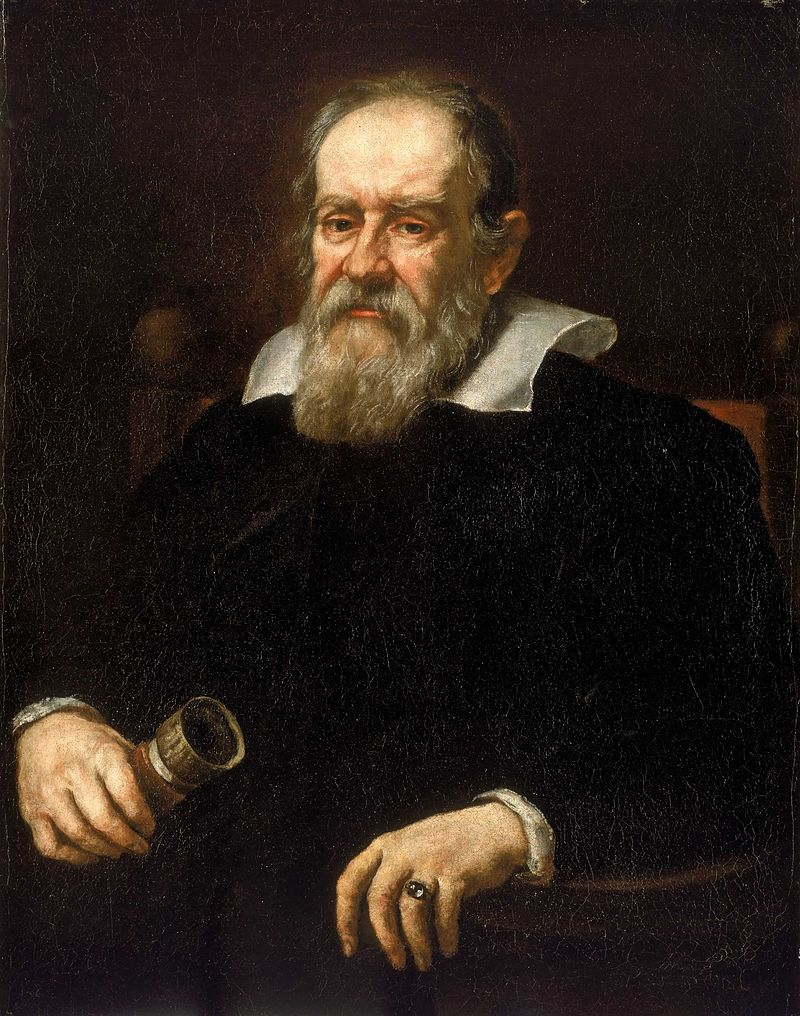
\includegraphics[width=0.8\textwidth]{Pictures/FFat/Galileo} 
		\end{column}
		\begin{column}{.6\textwidth}
			\only<2>{
			\begin{quotation}
			{\footnotesize 
				«La filosofia è scritta in questo grandissimo libro che continuamente ci sta aperto innanzi a gli occhi (io dico {\bf l'universo}), ma non si può intendere se prima non s'impara a intender la lingua, e conoscer i caratteri, ne' quali è scritto. 
				Egli {\bf è scritto in lingua matematica, e i caratteri son triangoli, cerchi, ed altre figure geometriche}, senza i quali mezzi è impossibile a intenderne umanamente parola; senza questi è un aggirarsi vanamente per un oscuro laberinto.»
			}
			\end{quotation}
			}
			\only<3->{		
			\begin{quotation}
			{\footnotesize 
				«Philosophy {\bf [nature]} is written in that great book which ever is before our eyes -- I mean the universe -- but we cannot understand it if we do not first learn the language and grasp the symbols in which it is written. 
				The book {\bf is written in mathematical language, and the symbols are triangles, circles and other geometrical figures}, without whose help it is impossible to comprehend a single word of it; without which one wanders in vain through a dark labyrinth.»		
			}
			\end{quotation}	
			}
			(Galileo Galilei, Il Saggiatore, 1623)	
		\end{column}	
	\end{columns}	
\end{frame}
\note[itemize]{
	\item Praticamente l'idea è vecchia quanto la scienza.f
}
%-------------------------------------------------------------------------------------------------------------------------------------------------


%-------------------------------------------------------------------------------------------------------------------------------------------------
\begin{frame}{What we mean by: \emph{Geometric mechanics}? (2)}
	What we mean \underline{here} is:
	\\
	the modern discipline originated in the 60s by the work of these mathematicians%gentlemen
	
	\vfill
	\begin{columns}[T]
		\begin{column}{.2\textwidth}
			\center
			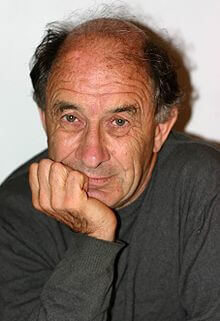
\includegraphics[width=0.8\textwidth]{Pictures/FFat/arnold}
			Vladimir \\ 
			Arnold
		\end{column}
		\begin{column}{.2\textwidth}
			\center
			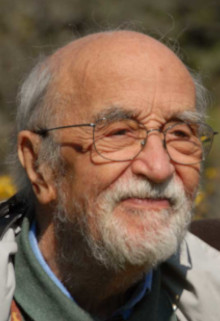
\includegraphics[width=0.8\textwidth]{Pictures/FFat/souriau} 
			Jean-Marie \\			
			Souriau
		\end{column}
		\begin{column}{.2\textwidth}
			\center
			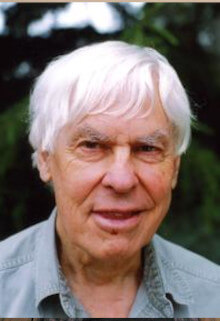
\includegraphics[width=0.8\textwidth]{Pictures/FFat/smale}
			Stephen \\
			Smale
		\end{column}
		\begin{column}{.2\textwidth}
			\center
			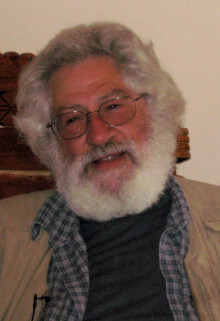
\includegraphics[width=0.8\textwidth]{Pictures/FFat/abraham} 
			Ralph \\			
			Abraham
		\end{column}
		\begin{column}{.2\textwidth}
			\center
			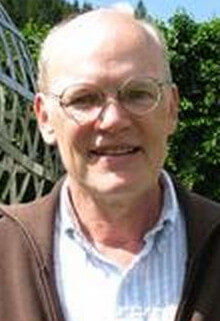
\includegraphics[width=0.8\textwidth]{Pictures/FFat/marsden} 
			Jerrold \\
			Marsden
		\end{column}		
	\end{columns}	

	\pause
	\vfill
	\begin{block}<1->{Introduced as a branch of \emph{(applied) Mathematics}}
			Employs modern (differential) geometry to the description of dynamical systems.	
	\end{block}


\end{frame}
\note[itemize]{
	\item %\href{https://en.wikipedia.org/wiki/Geometric_mechanics#History}{wiki}
		Arnold's fundamental work showed that Euler's equations for the free rigid body are the equations for geodesic flow on the rotation group SO(3) and carried this geometric insight over to the dynamics of ideal fluids, where the rotation group is replaced by the group of volume-preserving diffeomorphisms. 
	\item Smale's paper on Topology and Mechanics investigates the conserved quantities arising from Noether's theorem when a Lie group of symmetries acts on a mechanical system, and defines what is now called the momentum map (which Smale calls angular momentum), and he raises questions about the topology of the energy-momentum level surfaces and the effect on the dynamics. 
	\item Souriau also considered the conserved quantities arising from the action of a group of symmetries, but he concentrates more on the geometric structures involved (for example the equivariance properties of this momentum for a wide class of symmetries), and less on questions of dynamics.
	\item These ideas leads to the seminal book: \emph{Foundations of Mechanics} by Abraham and Marsden (1978).
	\item 		{physical è un po' restrittivo, diciamo sistemi che evolvono?}	
		{dynamical systems: non solo meccanica classica non relativistica non quantistica!}

}
%-------------------------------------------------------------------------------------------------------------------------------------------------

%-------------------------------------------------------------------------------------------------------------------------------------------------
\begin{frame}[t]{What is... \emph{Geometric Mechanics?}}
		\begin{block}{As an approach to \emph{Rational Mechanics}:}
			\begin{itemize}
				\item \textbf{Key idea:} make use of geometry to completely encode a physical system's mechanical properties regardless of the coordinate system employed.
				\item \textbf{The goal:} reconstruction of the physical observable quantities of interest from this abstract mathematical setting.
				\item \textbf{Advantages:} formalize the system's relevant structure in order to:
					\begin{itemize}
						\item[-] simplify the analytical or numerical solution of motion equations;
						\item[-] derive its quantum or relativistic counterpart.		
					\end{itemize}									
			\end{itemize}
		\end{block}
		%
		\vfill
		\pause
		\begin{block}{Some direct applications:}
			\vspace{-0.5em}
			\begin{columns}
		    	\begin{column}{.45\textwidth}
					\begin{itemize}
						\item[-] Theoretical chemistry
						\item[-] Control theory
						\item[-] Image processing
					\end{itemize}
				\end{column}
		    	\begin{column}{.45\textwidth}
					\begin{itemize}
						\item[-] Mathematical finance
						\item[-] Earth sciences
						\item[-] Robotics
					\end{itemize}
				\end{column}
			\end{columns}
		\end{block}
		\vfill
		\pause
		\begin{block}{Three cornerstones of geometric mechanics}
	\begin{center}
		%\scalebox{.8}{%
		{
		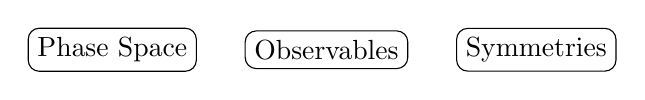
\begin{tikzpicture}[>=stealth,every node/.style={shape=rectangle,draw,rounded corners},node distance=0.05\linewidth,]
	    % create the nodes
		    \node (a1) {Phase Space};
		    \node (a2)[right =of a1] {Observables};
		    \node (a3)[right =of a2] {Symmetries};
		\end{tikzpicture}
%				\node [text width=0.6\linewidth, rectangle,draw,right of=lhs] (rhs) {Lie subgroup \\$G \subset Diff(M)$};
		}			
	\end{center}		
		\end{block}


		%https://en.wikipedia.org/wiki/Geometric_mechanics

		%http://www10.mathematik.uni-wuerzburg.de/index.php?path=research/maphy
	\end{frame}
	\note[itemize]{
		\item the geometric language permits to formalize the evolution of system composed of both quantum and classical degree of freedom (mesoscopic scale)
		\item Lessig: 
		In our discussion we only considered classical mechanical systems. However,
the theory applies to a diverse array of fields and disciplines ranging from quantum mechanics at the smallest scales to relativistic astrophysics at the largest, and applications can be found in areas such as image processing, space mission design, marine animal propulsion, mathematical finance, rising eggs, oceanography, plasma physics, falling cat phenomena, and many more. In its contemporary formulation using the rich toolbox of modern geometry, geometric mechanics provides thereby a surprisingly unified perspective on all these systems.
		\item Manifolds arise naturally in the description of classical mechanical systems.
		\item Geometrization of mechanics yields an inherent intuition to differential geometry structures (manifolds, charts, vectors ...).
		\item Encoding a classical mechanical system via a precise mathematical framework allows  to the relevant structures of our physical theories to emerge.
		\item A sound mathematical foundation provides a solid ground where to perform axiomatization of physical theories, quantization and "relativization".
		\item With a slight refinement of the mathematical language, also systems with continuous degrees of freedom (fluid and fields) can be accommodated within this geometrical framework as well.
		\item This framework could be adapted directly to ordinary quantum mechanical systems (e.g. Bloch sphere).
		\item There are also  direct applications!!! (if you are that kind of person .... :P )
				(if aiming to a complete mathematical foundation it's not enough for you...)
	}
%-------------------------------------------------------------------------------------------------------------------------------------------------


\end{document}